\documentclass[11pt]{beamer}
\usepackage[utf8]{inputenc}
\usepackage[T1]{fontenc}
\usepackage{lmodern}
\usepackage[english]{babel}
\usepackage{amsmath}
\usepackage{amsfonts}
\usepackage{amssymb}
\usepackage{graphicx}
\usetheme{AnnArbor}
\begin{document}
	\author[Soham, Sukhmani, Tarun, Ali]{Soham Sarfare \and Sukhmani Arora \and Tarun Tirupati \and Ali Saeed}
	\title[RetinaFace]{ RetinaFace: Single-stage Dense Face Localisation in the Wild}
	\subtitle{Application of Data Science - Final Project Presentation Group F}
	%\logo{\includegraphics[height=1.0cm]{logo.png}}
	\institute[]{Faculty of Computing \\ Macquarie University}
	%\date{}
	%\subject{}
	%\setbeamercovered{transparent}
	%\setbeamertemplate{navigation symbols}{}
	\begin{frame}[plain]
		\maketitle
	\end{frame}
	\begin{frame}
		\frametitle{Results on Original Data}
		\begin{itemize}
			\item Original code for the paper was obtained from the github repository made for the paper. The repository can be found at \url{https://github.com/deepinsight/insightface/tree/master/RetinaFace}. 
			\item Original WiderFace dataset was obatined from the website of the WiderFace Challenge. \url{http://shuoyang1213.me/WIDERFACE/} 
			\item The data along with the code was uploaded to google drive and executed via Colab.
			\item Testing the pretrained model on this data resulted in Average Precision scores similar to those obtained by the authors. The graphs below on easy, medium and hard validation sets are Precision-Recall curves per image and the highlighted values attest to the findings. 			
		\end{itemize}
	\end{frame}
\begin{frame}
	\frametitle{Results on Original Data}
	\begin{figure}
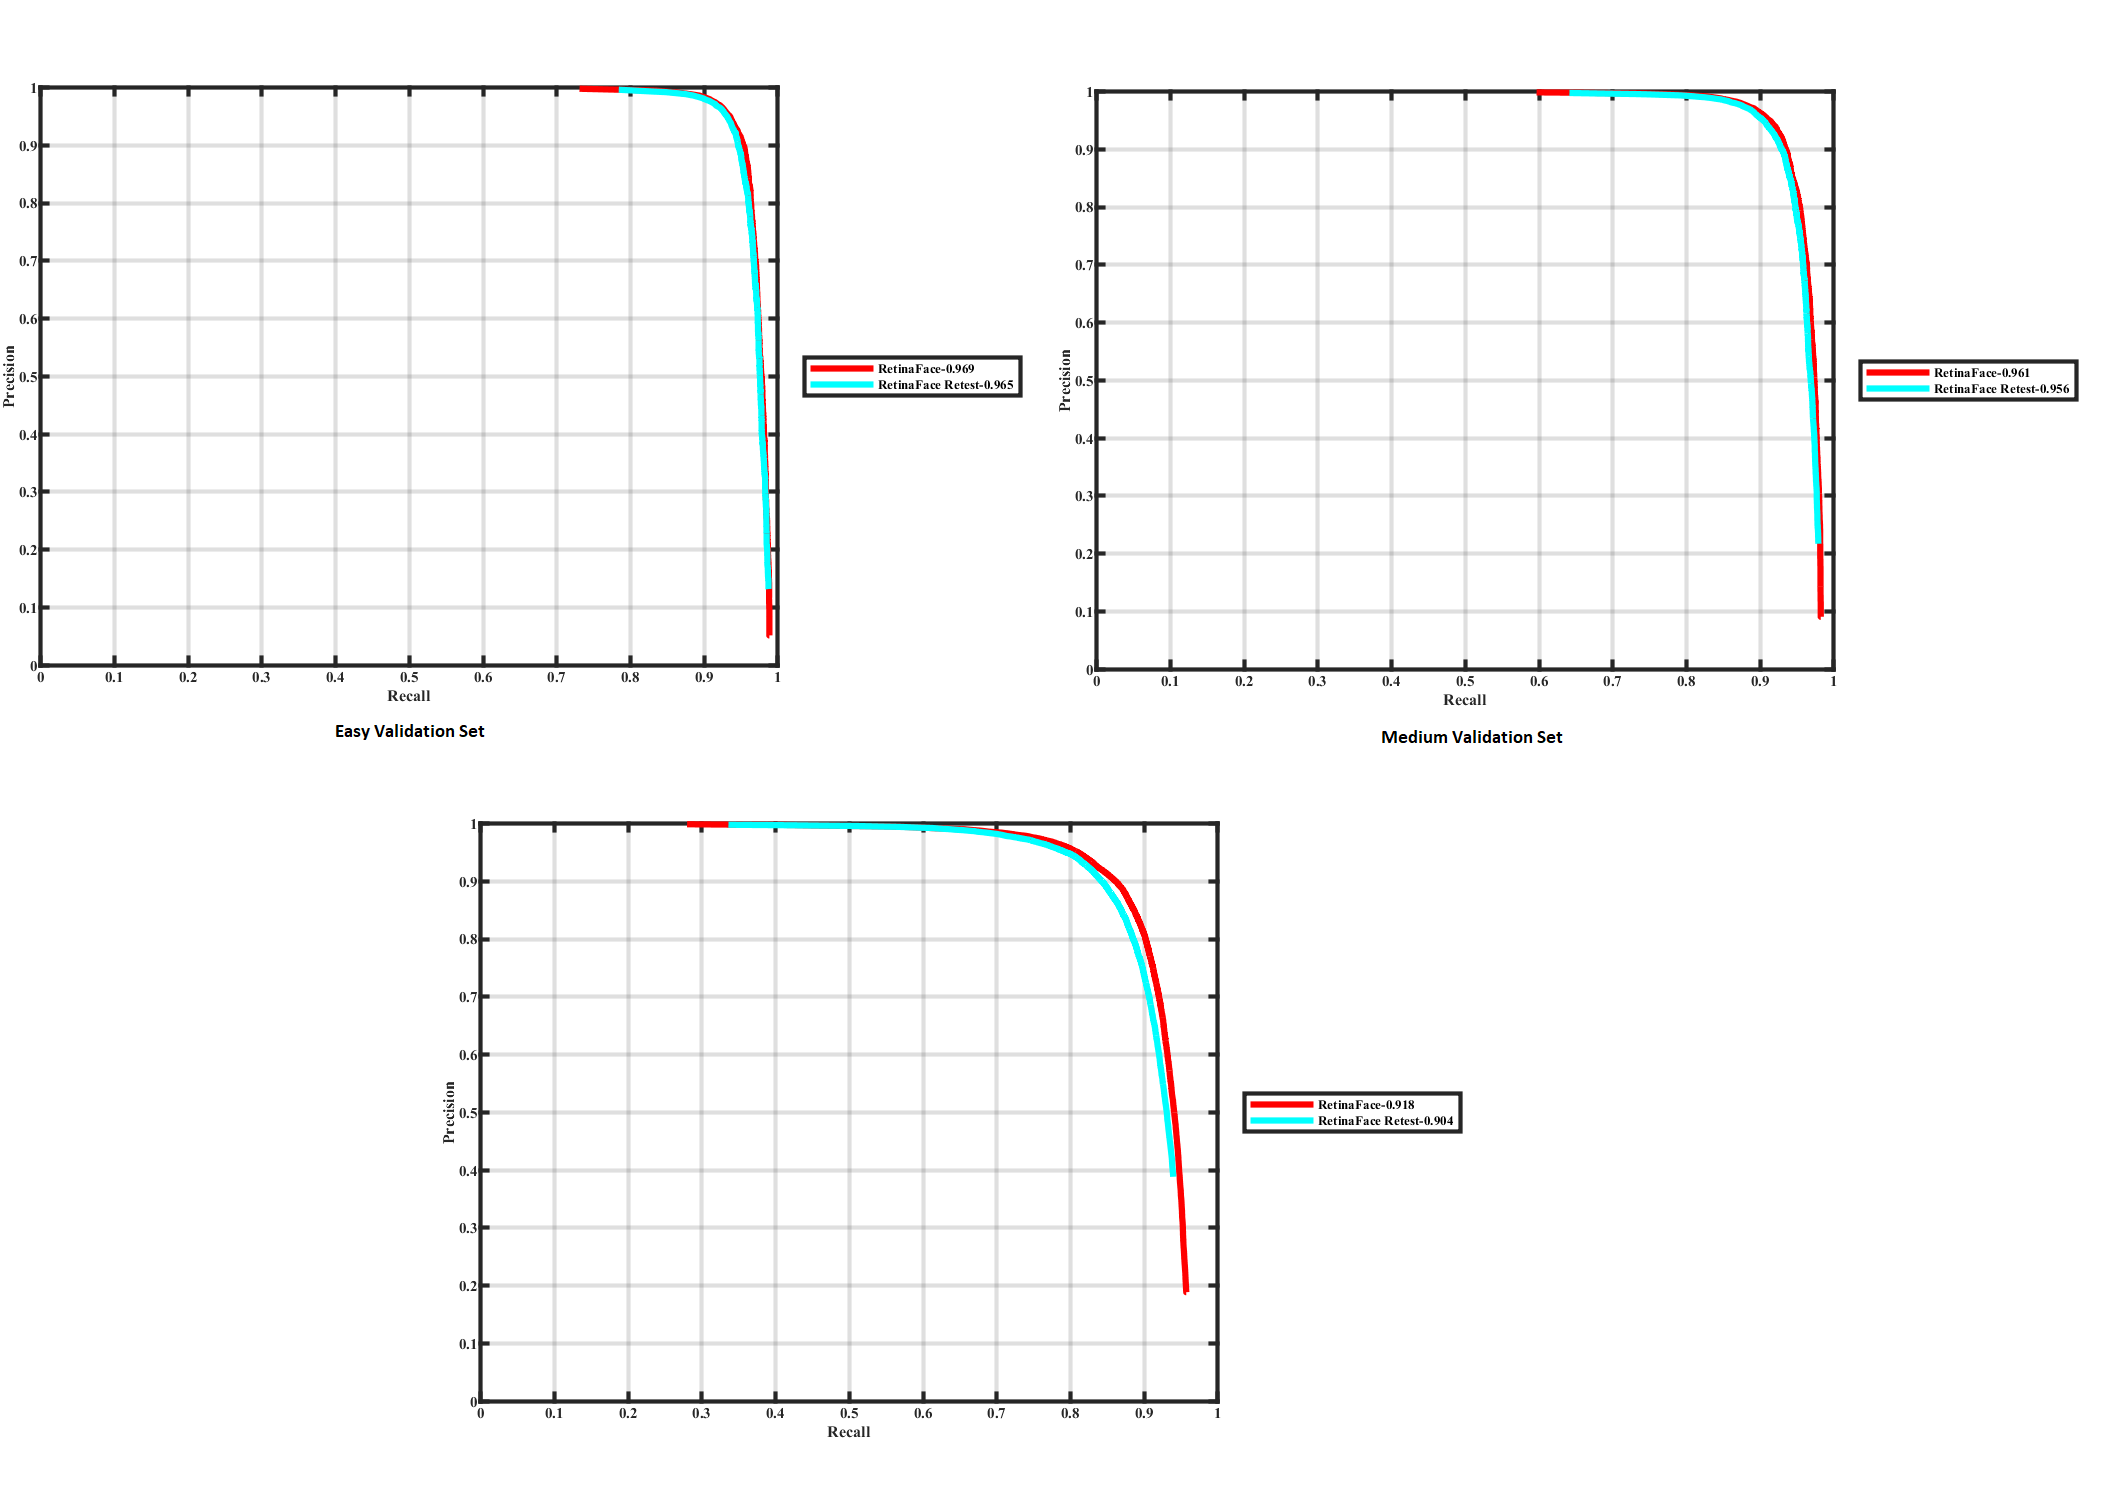
\includegraphics[width=0.75\linewidth]{final_out.png}
\caption{PR curves and corresponding MAP values}
		\end{figure}
	\end{frame}
\begin{frame}
\frametitle{Issues Faced}
\begin{itemize}
\item The size of the data was 3.5GB. The first challenge was to download the dataset and upload it to the drive.
\item None of the team members had any linux based machines and it was not possible to do this in a virtual environment(e.g. Virual Box) since it would be time-taking to test the entire dataset. Therefore, google colab was used with GPU.
\item More than six hours were taken by colab to test the entire dataset , hence we had to figure out a method to stop colab from timing out due to inactivity. This was achieved by running a JS function in the browser console. 
\item The process of verifying our findings was complicated since the evaluation method involved executing MATLAB files downloaded from the WIDERFACE website. This produced the graphs above along with the mAP scores. 
\end{itemize}
\end{frame}
\begin{frame}
	\frametitle{New Dataset}
	\begin{itemize}
\item Our aim was to collect new data that is similar to original dataset in order to obtain equivalent results as produced in the paper. Hence we have chosen the process of scraping images using google search engine and the process of web scraping images from a few websites.
\item The new dataset in arranged in such a way that the image data has a high degree of variability in scale, pose, expression, occlusion and illumination.
	\end{itemize}
\end{frame} 
\begin{frame}
	\frametitle{New Dataset}
\begin{itemize}
	
\item We have manually annotated 100 images by drawing a bounding box coordinates using Microsoft Paint in accordance to the outlines specified for the WiderFace dataset. 
\item The annotations have been written into text file in the form of (x,y) bounding box coordinates, breadth and length of bounding box. 
\item The new dataset is run through the code and evaluation results are observed and documented to check for similarity with original data results.

	\end{itemize}
\end{frame} 
\end{document}